\chapter{One usage -ou}
	
	Having know that one action can be applied at most once is useful information in some cases. Let say that there is an action $a_c$ with effect $<w_i,w_j>$, no other action needs $w_i$ and there are also at least one action action having opposite effect ($<w_j,w_i>$). In such case, an cycle composed from facts $w_i$, $w_j$ and those actions is created. Now, our aim is to destroy such a cycle because it can further simplify the problem or another reduction may be applied. 
	
	The reduction itself is based on adding one new fact $w_n$ instead of $w_i$ or $w_j$ in one of the effects; so, either $<w_i,w_j>$ is replaced by $<w_i,w_n>$ or $<w_j,w_i>$ is replaced by $<w_j,w_n>$. The procedure when $w_i$ or $w_j$ is replaced is described further in reduction description.
	
	While doing this reduction, two things should be taken in mind. Firstly, effect cannot be removed from action and replaced by prevail precondition, since delete relaxation could occur; this may for example happen when there are multiple actions having the opposite effect to $a_c$. Secondly, there must not be any action needing the fact that is being replaced (only $a_c$ can need the fact).
	
	
	\section{Reduce operation}
	Let's have SAS in form $<\vars, \init, \goal, \actions, \mutexes{}>$. 
	
	This operation is executed if there is $u_i$, $u_j$, $a_c$, $a_d$, $w_i$ and $w_j$ such that:
	
	\begin{enumerate}
		\item $u_i \in \init$ \label{ou:in:ai:invariantStart}
		\item $|\con{u_i}| > 0$ 
		\item $|\pro{u_i}| = 0$ 
		\item $a_c \in \con{u_i}$ 
		\item $<u_i,u_j> \in \eff{a_c}$ 
		\item $|\con{u_j}| = 0$ \label{ou:in:ai:invariantEnd}
		\item $<w_i,w_j> \in \eff{a_c}, \var{w_i} \neq \var{v_i}$; action $a_c$ has another effect
		\item $|\pro{w_i}| = |\con{w_j}| = |\{a | <w_j,w_i> \in \eff{a}, a \in \actions \}|$ \label{ou:in:onlyActionWithOppositeEffect}
		\item $|\wan{w_i}| = 1$ \label{ou:in:noPre}
		\item $a_d \in \con{w_j}$
		\item $<w_j,w_i> \in \eff{a_d}$
		\item $|\con{w_i}| = 1$
	\end{enumerate}
	
	Action $a_c$ can be applied at most once (\ref{ou:in:ai:invariantStart} - \ref{ou:in:ai:invariantEnd}). Moreover, $a_c$ has another effect $<w_i,w_j>$. So, if there is another action $a_d$ having effect $<w_j,w_i>$, which is opposite to the effect of $a_c$, then the reduction may be executed. In the case that there would be more consumers of $w_j$ than one, then the effect $<w_j,w_i>$ cannot be removed, since delete relaxation could rise.
	
	\ref{ou:in:onlyActionWithOppositeEffect} tells that if there is action having $w_j$ in delete effect, then it also must have $w_i$ in add effect. Also there may exist action having $w_i$ in prevail precondition. But there cannot be any other action than $a_c$ having $w_i$ in prevail preconditions nor delete effects.
	
	The operation does following things:
	
	Case A: $w_i \in \init$
		\begin{enumerate}
			\item $\dom{\var{w_i}} = \dom{\var{w_i}} \cup \{w_n\}$
			\item for each action $a_d$ having effect $a_d' \leftarrow <\pre{a_d},(\eff{a_d} \setminus \{<w_j,w_i>\}) \cup \{<w_j,w_n>\}>$, $\actions{}' \leftarrow ((\actions' \cup \actions) \setminus a_d) \cup \{a_d'\}$ 
		\end{enumerate}	
	
	\begin{figure}
		\begin{subfigure}[b]{0.4\textwidth}
			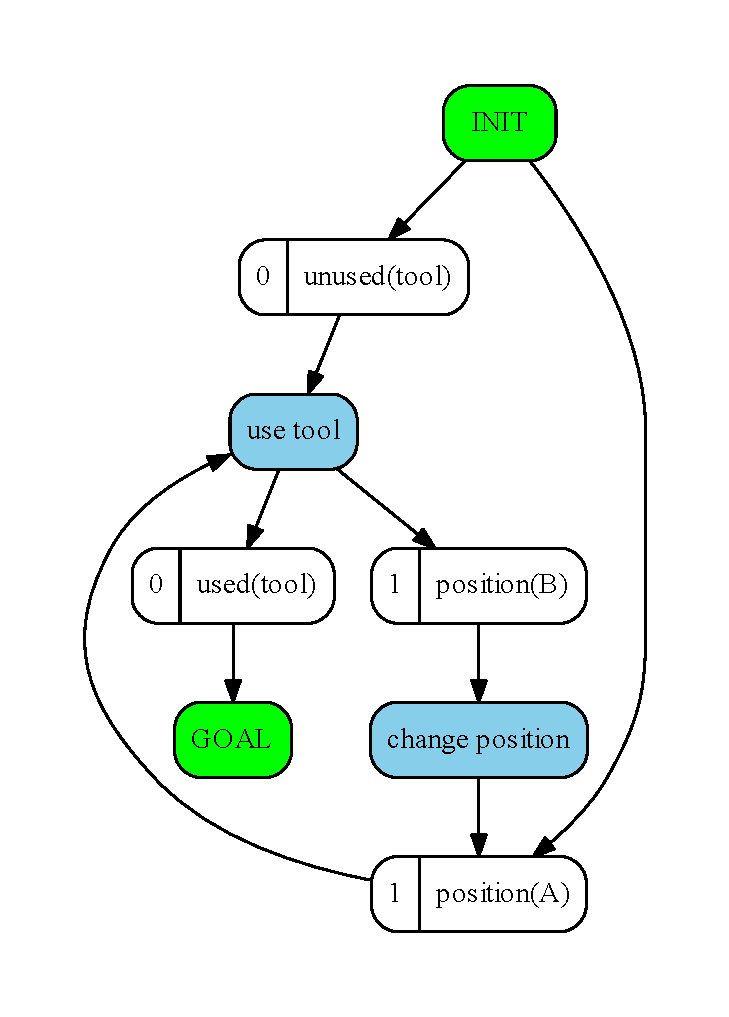
\includegraphics[scale=0.4]{oneUsage/figures/startsInInit_input}
			\caption{before reduction}
		\end{subfigure}	
		\begin{subfigure}[b]{0.4\textwidth}
			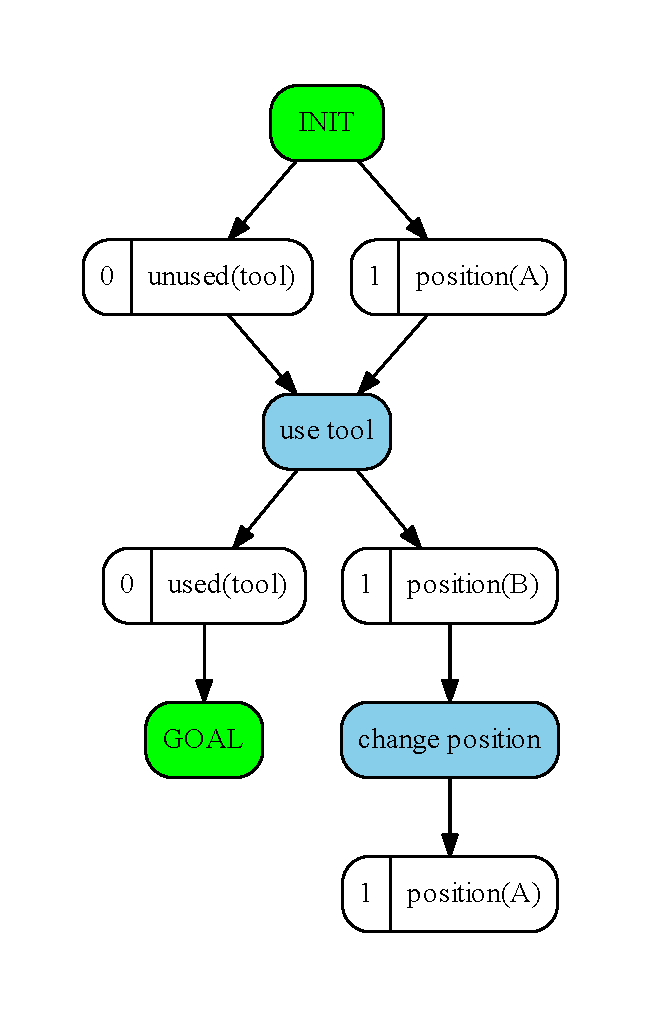
\includegraphics[scale=0.4]{oneUsage/figures/startsInInit_output}
			\caption{after reduction}
		\end{subfigure}
		\caption{case A: $w_i \in \init$; $\var{w_j} = $ variable 1, $\var{u_j}$ = variable 0, $a_c$ = \emph{use tool}, $a_d = $ \emph{change position}, $w_i = $ \emph{1 position B}}
	\end{figure}
	
	
	Case B: $w_j \in \init$
	
	\begin{enumerate}
		\item $\dom{\var{w_i}} = \dom{\var{w_i}} \cup \{w_n\}$
		\item $a_c' \leftarrow <\pre{a_c},(\eff{a_c} \setminus \{<w_i,w_j>\}) \cup \{<w_i,w_n>\}>$, 
		\item $\actions{}' \leftarrow (\actions \setminus \{a_c\}) \cup \{a_c'\}$ 
	\end{enumerate}		
	
	
	\begin{figure}
		\begin{subfigure}[b]{0.4\textwidth}
			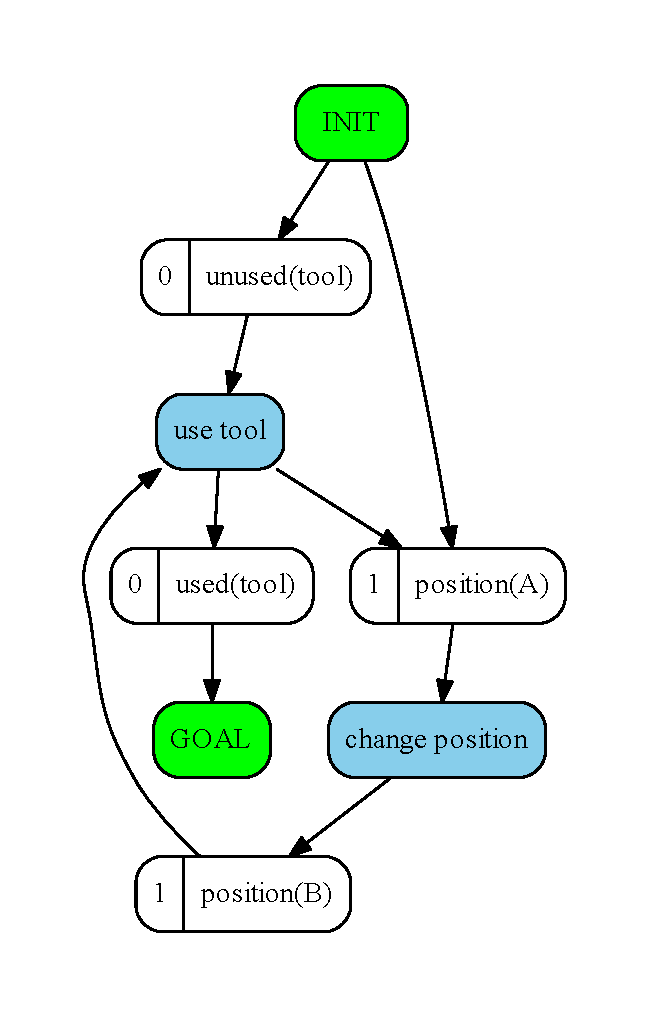
\includegraphics[scale=0.4]{oneUsage/figures/endsInInit_input}
			\caption{before reduction}
		\end{subfigure}	
		\begin{subfigure}[b]{0.4\textwidth}
			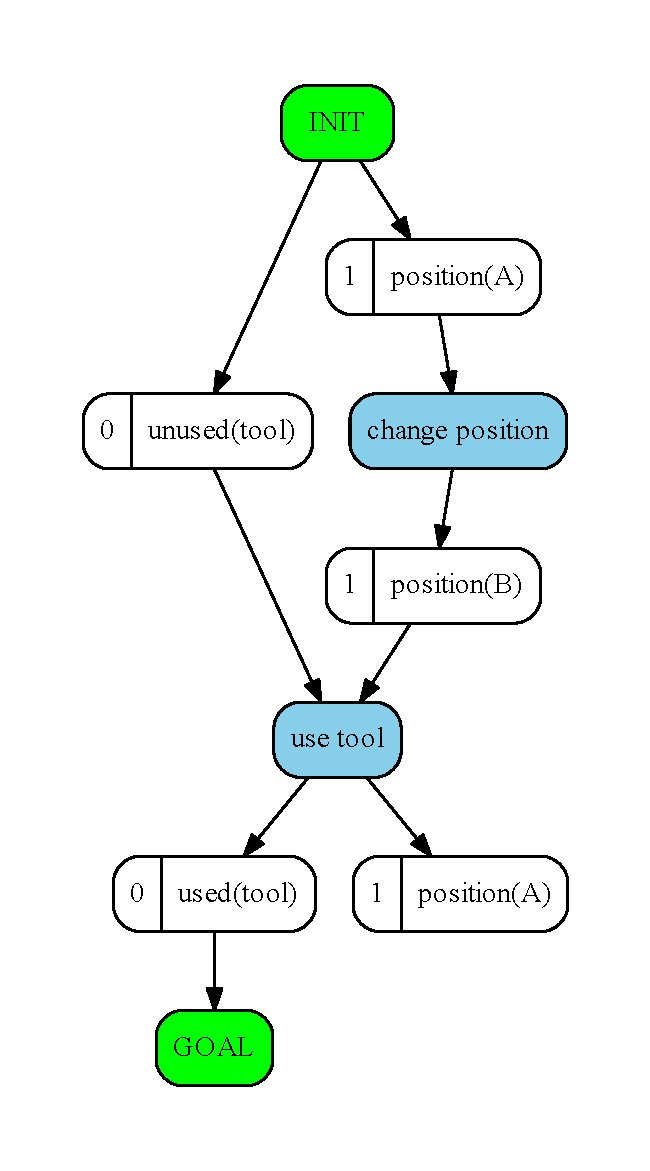
\includegraphics[scale=0.4]{oneUsage/figures/endsInInit_output}
			\caption{after reduction}
		\end{subfigure}
		\caption{case B: $w_j \in \init$; $\var{w_j} = $ variable 1, $\var{u_j}$ = variable 0, $a_c$ = \emph{use tool}, $a_d = $ \emph{change position}, $w_j = $ \emph{1 position A}}		
	\end{figure}
	
	
	Output of the reduction is SAS $<\vars{}', \init{}, \goal{}, \actions{}', \mutexes{}>$.
	
	
	\section{Possible outgoing states of SAS}
	\begin{enumerate}
		\item application of -oe, -sf, -ai
	\end{enumerate}
	
	After implementing this reduction, other reduction were implemented; namely -sf or -ai could be doing some operation with the SAS that this reduction may become redundant in some cases.
	
	\section{States before application of this operation}
	\begin{itemize}
		\item from the beginning
		\item after application of -sd, -hc, -mo, maybe others (does not which right now)
	\end{itemize}
	
	
	\section{Reverse operation}
	During the reverse operation, effect of type $<w_i,w_n>$ are replaced back by $<w_i,w_j>$ and $<w_j,w_n>$ are replaced back by $<w_j,w_i>$. No extension of the plan is done.
	
	\section{Implementation notes}
	Now, it returns multi reverse operation.
	
	There is some bug. Only thing I came up with is that in current implementation, there are no such strict condition over set of consumers and producers. If the bug is not hidden inside these condition, then I would revise method Operation.isProducing(value) if the -1 value is used without mistakes. There is also possibility that implementation does not contain check for $w_i$ or $w_j$ to be in $\init$.
	
	The name of newly added fact is quite unimportant. In the implementation, there the name is get as copy of the fact that is being replaced. This is because preprocess of FD is parsing names of facts (so it cares about predicate names, etc, somehow). Also it should be run before -uv.
	
